\documentclass{article}
\usepackage{graphicx} % Required for inserting images
\usepackage{geometry}
\usepackage{circuitikz}
\usepackage{siunitx}
\usepackage{CJKutf8}
\usepackage{amsmath}
\usepackage{amssymb}
\usepackage{caption}
\usepackage{float}
\usepackage{subcaption}
\geometry{top=10mm, left=20mm, a4paper}
\title{Feddback Circuit Active Filter Report}
\author{梁程捷(B11901136),吳奕娃(B11901080)}
\date{}

\begin{document}
\begin{CJK*}{UTF8}{bkai}
\maketitle

%============Differential Amplifier====================
\section*{Band Pass Filter}
\begin{minipage}{0.5\textwidth}
\begin{table}[H]
\begin{tabular}{|c|c|c||c|c|c|}
    \hline
    $f$ (\unit{\kilo\hertz}) &  $V_i$ (V)& $V_o$ (V) & $f$ (\unit{\kilo\hertz}) &  $V_i$ (V)& $V_o$ (V)\\
    \hline\hline
    0.5	    & 2.040 & 0.12 & \textbf{\underline{{15}}} & \textbf{\underline{{0.360}}} & \textbf{\underline{{1.32}}}   \\
    1       & 2.060 & 0.22 & 18     & 0.360 & 1.20  \\
    2	    & 2.040 & 0.42 & 19     & 0.560 & 1.70  \\
    3	    & 2.040 & 0.63 & 20     & 0.560 & 1.52   \\
    5	    & 1.640 & 1.08 & 20.5   & 0.490 & 1.24   \\
    10	    & 0.940 & 1.58 & 21     & 0.560 & 1.36   \\
    12	    & 0.340 & 0.86 & 25     & 0.540 & 0.96   \\
    12.5	& 0.480 & 1.30 & 30     & 0.540 & 0.74   \\
    13      & 0.340 & 1.02 & 40     & 0.480 & 0.52   \\
    14      & 0.340 & 1.18 &        &       &        \\
\hline
\end{tabular}
\caption{raw experimental data}
\end{table}
\end{minipage}\hspace{20mm}
\begin{minipage}{0.5\textwidth}
    \begin{figure}[H]    
        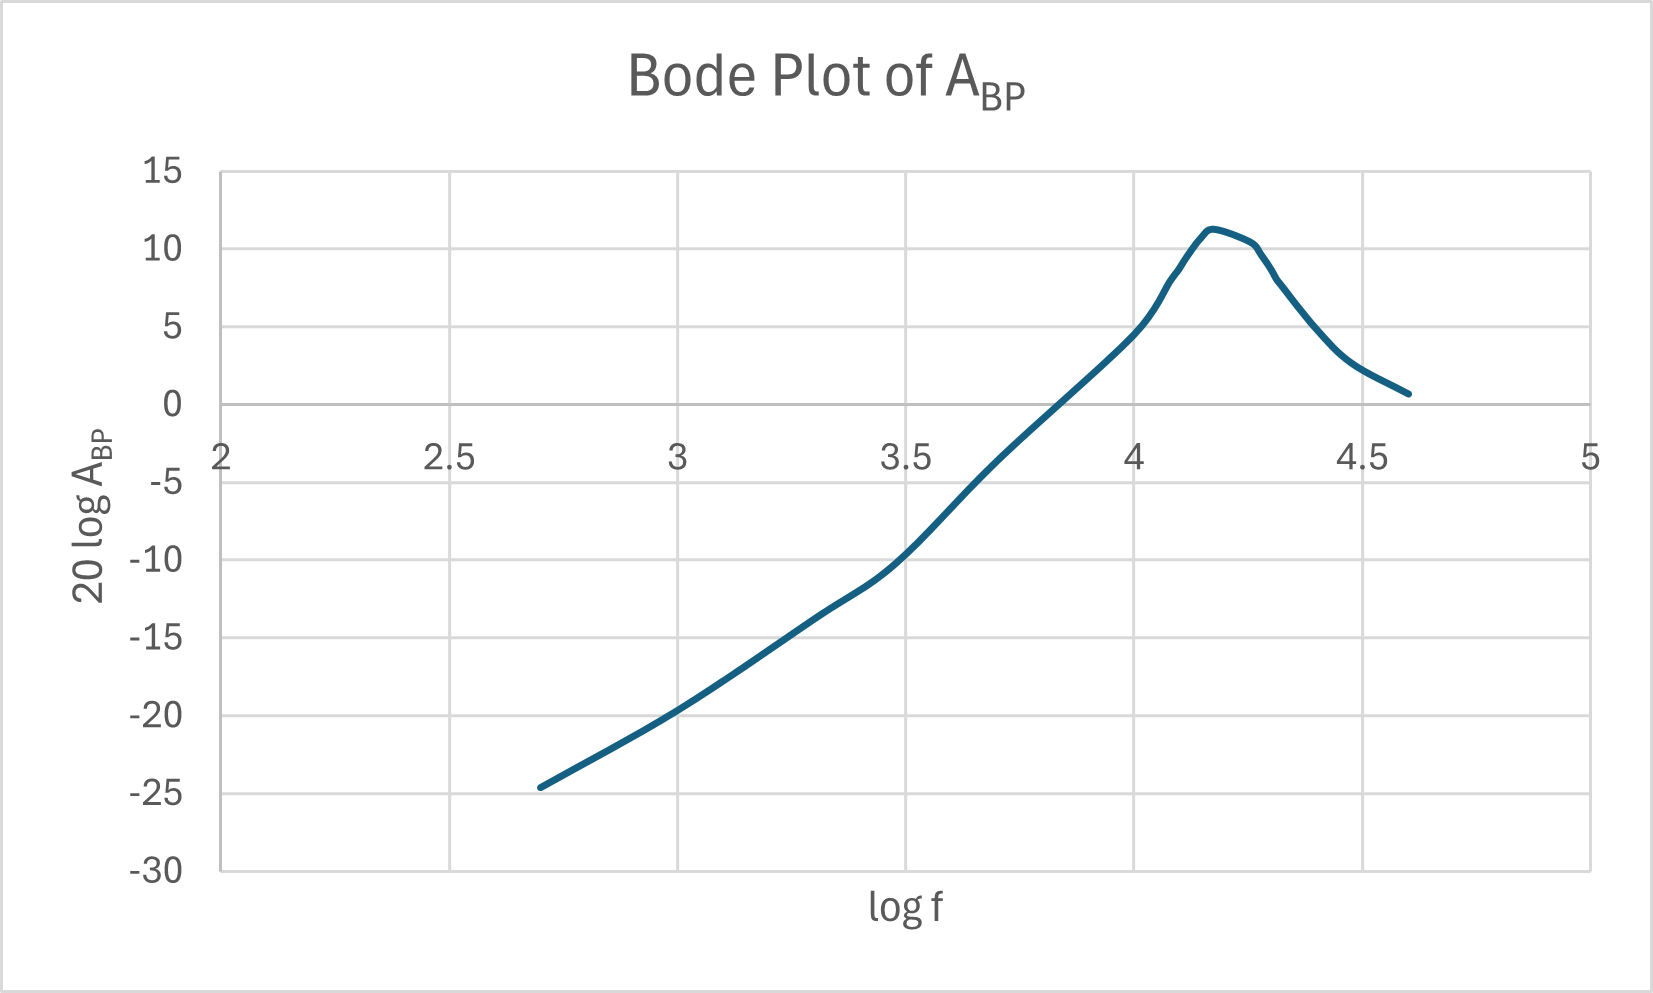
\includegraphics[scale=0.55]{Abp_bode_plot.png}
        \caption{Bode Plot of $A_{BP}$}
    \end{figure}
\end{minipage}
\vspace{3mm}\\
\textbf{Maximum voltage gain $A_{max} = \frac{1.32}{0.36}$ = 3.67 V/V}, \textbf{$f_{L3dB,BP}$ = 12 \unit{\kilo\hertz}}, \textbf{$f_{H3dB,BP}$ = 20.5 \unit{\kilo\hertz}},\\
\vspace*{1mm}\\
\textbf{Bandwidth BW = 20.5 - 12 = 8.5 \unit{\kilo\hertz}}

\section*{Reflections}
\subsection*{梁程捷}
這次實驗的電路比較複雜,電線相互交錯,有時電阻還不小心短路,接了好幾次才成功,下次實驗要多練幾次。
\subsection*{吳奕娃}
這次的實驗感覺比以往困難不少,花了很多時間才做完,希望之後有機會練習以熟悉電路的接法。
\end{CJK*}
\end{document}
